% Options for packages loaded elsewhere
\PassOptionsToPackage{unicode}{hyperref}
\PassOptionsToPackage{hyphens}{url}
\PassOptionsToPackage{dvipsnames,svgnames,x11names}{xcolor}
%
\documentclass[
]{agujournal2019}

\usepackage{amsmath,amssymb}
\usepackage{iftex}
\ifPDFTeX
  \usepackage[T1]{fontenc}
  \usepackage[utf8]{inputenc}
  \usepackage{textcomp} % provide euro and other symbols
\else % if luatex or xetex
  \usepackage{unicode-math}
  \defaultfontfeatures{Scale=MatchLowercase}
  \defaultfontfeatures[\rmfamily]{Ligatures=TeX,Scale=1}
\fi
\usepackage{lmodern}
\ifPDFTeX\else  
    % xetex/luatex font selection
\fi
% Use upquote if available, for straight quotes in verbatim environments
\IfFileExists{upquote.sty}{\usepackage{upquote}}{}
\IfFileExists{microtype.sty}{% use microtype if available
  \usepackage[]{microtype}
  \UseMicrotypeSet[protrusion]{basicmath} % disable protrusion for tt fonts
}{}
\makeatletter
\@ifundefined{KOMAClassName}{% if non-KOMA class
  \IfFileExists{parskip.sty}{%
    \usepackage{parskip}
  }{% else
    \setlength{\parindent}{0pt}
    \setlength{\parskip}{6pt plus 2pt minus 1pt}}
}{% if KOMA class
  \KOMAoptions{parskip=half}}
\makeatother
\usepackage{xcolor}
\setlength{\emergencystretch}{3em} % prevent overfull lines
\setcounter{secnumdepth}{5}
% Make \paragraph and \subparagraph free-standing
\makeatletter
\ifx\paragraph\undefined\else
  \let\oldparagraph\paragraph
  \renewcommand{\paragraph}{
    \@ifstar
      \xxxParagraphStar
      \xxxParagraphNoStar
  }
  \newcommand{\xxxParagraphStar}[1]{\oldparagraph*{#1}\mbox{}}
  \newcommand{\xxxParagraphNoStar}[1]{\oldparagraph{#1}\mbox{}}
\fi
\ifx\subparagraph\undefined\else
  \let\oldsubparagraph\subparagraph
  \renewcommand{\subparagraph}{
    \@ifstar
      \xxxSubParagraphStar
      \xxxSubParagraphNoStar
  }
  \newcommand{\xxxSubParagraphStar}[1]{\oldsubparagraph*{#1}\mbox{}}
  \newcommand{\xxxSubParagraphNoStar}[1]{\oldsubparagraph{#1}\mbox{}}
\fi
\makeatother


\providecommand{\tightlist}{%
  \setlength{\itemsep}{0pt}\setlength{\parskip}{0pt}}\usepackage{longtable,booktabs,array}
\usepackage{calc} % for calculating minipage widths
% Correct order of tables after \paragraph or \subparagraph
\usepackage{etoolbox}
\makeatletter
\patchcmd\longtable{\par}{\if@noskipsec\mbox{}\fi\par}{}{}
\makeatother
% Allow footnotes in longtable head/foot
\IfFileExists{footnotehyper.sty}{\usepackage{footnotehyper}}{\usepackage{footnote}}
\makesavenoteenv{longtable}
\usepackage{graphicx}
\makeatletter
\def\maxwidth{\ifdim\Gin@nat@width>\linewidth\linewidth\else\Gin@nat@width\fi}
\def\maxheight{\ifdim\Gin@nat@height>\textheight\textheight\else\Gin@nat@height\fi}
\makeatother
% Scale images if necessary, so that they will not overflow the page
% margins by default, and it is still possible to overwrite the defaults
% using explicit options in \includegraphics[width, height, ...]{}
\setkeys{Gin}{width=\maxwidth,height=\maxheight,keepaspectratio}
% Set default figure placement to htbp
\makeatletter
\def\fps@figure{htbp}
\makeatother
% definitions for citeproc citations
\NewDocumentCommand\citeproctext{}{}
\NewDocumentCommand\citeproc{mm}{%
  \begingroup\def\citeproctext{#2}\cite{#1}\endgroup}
\makeatletter
 % allow citations to break across lines
 \let\@cite@ofmt\@firstofone
 % avoid brackets around text for \cite:
 \def\@biblabel#1{}
 \def\@cite#1#2{{#1\if@tempswa , #2\fi}}
\makeatother
\newlength{\cslhangindent}
\setlength{\cslhangindent}{1.5em}
\newlength{\csllabelwidth}
\setlength{\csllabelwidth}{3em}
\newenvironment{CSLReferences}[2] % #1 hanging-indent, #2 entry-spacing
 {\begin{list}{}{%
  \setlength{\itemindent}{0pt}
  \setlength{\leftmargin}{0pt}
  \setlength{\parsep}{0pt}
  % turn on hanging indent if param 1 is 1
  \ifodd #1
   \setlength{\leftmargin}{\cslhangindent}
   \setlength{\itemindent}{-1\cslhangindent}
  \fi
  % set entry spacing
  \setlength{\itemsep}{#2\baselineskip}}}
 {\end{list}}
\usepackage{calc}
\newcommand{\CSLBlock}[1]{\hfill\break\parbox[t]{\linewidth}{\strut\ignorespaces#1\strut}}
\newcommand{\CSLLeftMargin}[1]{\parbox[t]{\csllabelwidth}{\strut#1\strut}}
\newcommand{\CSLRightInline}[1]{\parbox[t]{\linewidth - \csllabelwidth}{\strut#1\strut}}
\newcommand{\CSLIndent}[1]{\hspace{\cslhangindent}#1}

\usepackage{url} %this package should fix any errors with URLs in refs.
\usepackage{lineno}
\usepackage[inline]{trackchanges} %for better track changes. finalnew option will compile document with changes incorporated.
\usepackage{soul}
\linenumbers
\makeatletter
\@ifpackageloaded{float}{}{\usepackage{float}}
\floatstyle{plain}
\@ifundefined{c@chapter}{\newfloat{suppfig}{h}{losuppfig}}{\newfloat{suppfig}{h}{losuppfig}[chapter]}
\floatname{suppfig}{Figure S}
\newcommand*\quartosuppfigref[1]{Figure \hyperref[#1]{S\ref{#1}}}
\@ifpackageloaded{caption}{}{\usepackage{caption}}
\DeclareCaptionLabelFormat{quartosuppfigreflabelformat}{#1#2}
\captionsetup[suppfig]{labelformat=quartosuppfigreflabelformat}
\newcommand*\listofsuppfigs{\listof{suppfig}{List of Supplementary Figures}}
\makeatother
\makeatletter
\@ifpackageloaded{caption}{}{\usepackage{caption}}
\AtBeginDocument{%
\ifdefined\contentsname
  \renewcommand*\contentsname{Table of contents}
\else
  \newcommand\contentsname{Table of contents}
\fi
\ifdefined\listfigurename
  \renewcommand*\listfigurename{List of Figures}
\else
  \newcommand\listfigurename{List of Figures}
\fi
\ifdefined\listtablename
  \renewcommand*\listtablename{List of Tables}
\else
  \newcommand\listtablename{List of Tables}
\fi
\ifdefined\figurename
  \renewcommand*\figurename{Figure}
\else
  \newcommand\figurename{Figure}
\fi
\ifdefined\tablename
  \renewcommand*\tablename{Table}
\else
  \newcommand\tablename{Table}
\fi
}
\@ifpackageloaded{float}{}{\usepackage{float}}
\floatstyle{ruled}
\@ifundefined{c@chapter}{\newfloat{codelisting}{h}{lop}}{\newfloat{codelisting}{h}{lop}[chapter]}
\floatname{codelisting}{Listing}
\newcommand*\listoflistings{\listof{codelisting}{List of Listings}}
\makeatother
\makeatletter
\makeatother
\makeatletter
\@ifpackageloaded{caption}{}{\usepackage{caption}}
\@ifpackageloaded{subcaption}{}{\usepackage{subcaption}}
\makeatother

\ifLuaTeX
  \usepackage{selnolig}  % disable illegal ligatures
\fi
\usepackage{bookmark}

\IfFileExists{xurl.sty}{\usepackage{xurl}}{} % add URL line breaks if available
\urlstyle{same} % disable monospaced font for URLs
\hypersetup{
  pdftitle={Regional-scale Base-flow Index of Gauged and Ungauged Basins in Drylands},
  pdfauthor={Caelum Mroczek; Abraham Springer; Benjamin Lucas},
  pdfkeywords={Base Flow, Base-flow Index, Regionalization, Machine
Learning},
  colorlinks=true,
  linkcolor={blue},
  filecolor={Maroon},
  citecolor={Blue},
  urlcolor={Blue},
  pdfcreator={LaTeX via pandoc}}


\journalname{Water Resources Research}

\draftfalse

\begin{document}
\title{Regional-scale Base-flow Index of Gauged and Ungauged Basins in
Drylands}

\authors{Caelum Mroczek\affil{1}, Abraham Springer\affil{1}, Benjamin
Lucas\affil{2}}
\affiliation{1}{School of Earth and Sustainability, Northern Arizona
University, Flagstaff, AZ, USA, }\affiliation{2}{Department of
Mathematics and Statistics, Northern Arizona University, Flagstaff, AZ,
USA, }
\correspondingauthor{Caelum Mroczek}{csm428@nau.edu}


\begin{abstract}
LOREM IPSUM \#\#\#\#\#\#
\end{abstract}

\section*{Plain Language Summary}
LOREM IPSUM \#\#\#\#\#\#




\section{Introduction}\label{sec-intro}

Dryland regions, encompassing arid, semi-arid, hyper-arid, and dry
sub-humid systems, account for 40\% of the Earth's land surface. These
regions are home to approximately 2 billion people globally and
constitute the largest terrestrial biome (IUCN, 2019). Despite
supporting diverse ecosystems and human populations, dryland regions
face mounting challenges exacerbated by increasing urbanization,
expanding agricultural activities, and climate-induced amplification of
precipitation patterns (Taylor et al., 2013). This water scarcity is
intensifying due to the compounding effects of climate variability and
increased groundwater extraction (Taylor et al., 2013). In drylands,
groundwater serves as a vital resource for sustaining ecosystems and
meeting human needs (Scanlon et al., 2006; Yao et al., 2018).

Base flow is the sustained portion of streamflow in the absence of
runoff that is derived from groundwater discharge (USGS, 2018). Base
flow is critical to maintaining seasonal low-flow regimes, supporting
aquatic ecosystems, and facilitating the transport of nutrients and
chemicals. Base-flow contribution to streamflow can be highly variable
spatially (Beck et al., 2013; Bosch et al., 2017; Singh et al., 2018),
and temporally (Ficklin et al., 2016; Tan et al., 2020). Increasing
groundwater extraction, changes in land cover/land use, and changes in
precipitation patterns due to climate change affect the timing and
volumes of base flow (Tan et al., 2020; Taylor et al., 2013). Effective
management of water quantity and quality depends on understanding
seasonal and interannual base flow patterns and long-term changes in
base flow behavior.

The Base-Flow Index (BFI) is the ratio of the long-term mean base-flow
volume to the long-term total streamflow volume expressed as a
percentage. BFI serves as a normalized measure of groundwater
contribution interannually or between basins. BFI is determined by
hydrograph separation and is influenced by the climate and physiographic
characteristics of a catchment (Beck et al., 2013; Neff et al., 2005;
Singh et al., 2018). Between catchments, base flow fluctuates according
to changes in the moisture content of the vadose zone, influenced by
varying levels of evapotranspiration and aquifer storage dynamics (Bosch
et al., 2017). Since BFI calculations rely on instrumented stream
records, it remains unknown for ungauged catchments, which encompass
most of the earth's land surface (Fekete et al., 2007). Addressing this
information gap is integral to approaching a comprehensive understanding
of groundwater dynamics globally.

To address the challenge of quantifying base flow in ungauged
catchments, numerous studies have applied regression and machine
learning methods. (Ahiablame et al., 2013) found that using a regression
model to estimate annual base flow of ungauged catchments was reasonably
easy and accurate. Beck et al. (2013) overcame the nonlinearity of basin
characteristics and improved results of multivariate analyses by using
artificial neural networks to estimate BFI globally. Singh et al. (2018)
implemented a random forest algorithm to predict long-term BFI for
ungauged catchments across New Zealand. The application of machine
learning in past studies highlights its versatility and effectiveness in
addressing ecohydrologic dynamics.

This study develops a technique for estimating BFI in ungauged basins in
Arizona and determines the state's long-term mean BFI. Using a machine
learning model trained with the hydrogeologic characteristics of surface
water basins, we estimate mean BFI in ungauged basins over a period of
record from 1991-2020. Regional patterns and trends in base flow and BFI
of instrumented sites are subsequently investigated. These results
provide novel analyses of low flow processes in Arizona, furthering our
understanding of climate controls on consistent flows in dryland basins.

\section{Data \& Methods}\label{sec-data-methods}

\subsection{Study Area}\label{sec-study-area}

The state of Arizona, located in the southwest United States, covers a
total area of 295,253 km\(^2\). Arizona is divided into two primary
physiographic provinces: the Colorado Plateau in the northeast, and the
Basin-and-Range region in the west and south. The Central Highlands is a
transition zone consisting of scattered basins separated by the
mountainous foothills of the Mogollon Rim. The Colorado Plateau is
dominated by high-elevation desert with an average elevation of 1,936
masl (6,352 ft). Mean temperatures range from -6\(^\circ\)C
(20\(^\circ\)F) to 26\(^\circ\)C (80\(^\circ\)F) and it averages 580 mm
(23 in) of precipitation. The Basin-and-Range region has a semi-arid to
arid climate with an average elevation of 490 masl (1600 ft). Average
temperature ranges from 15\(^\circ\)C (60\(^\circ\)F) to 43\(^\circ\)C
(110\(^\circ\)F) and the region averages 200 mm (8 in) of precipitation
annually. \#\#\#CITATION\#\#\#

\begin{figure}

\centering{

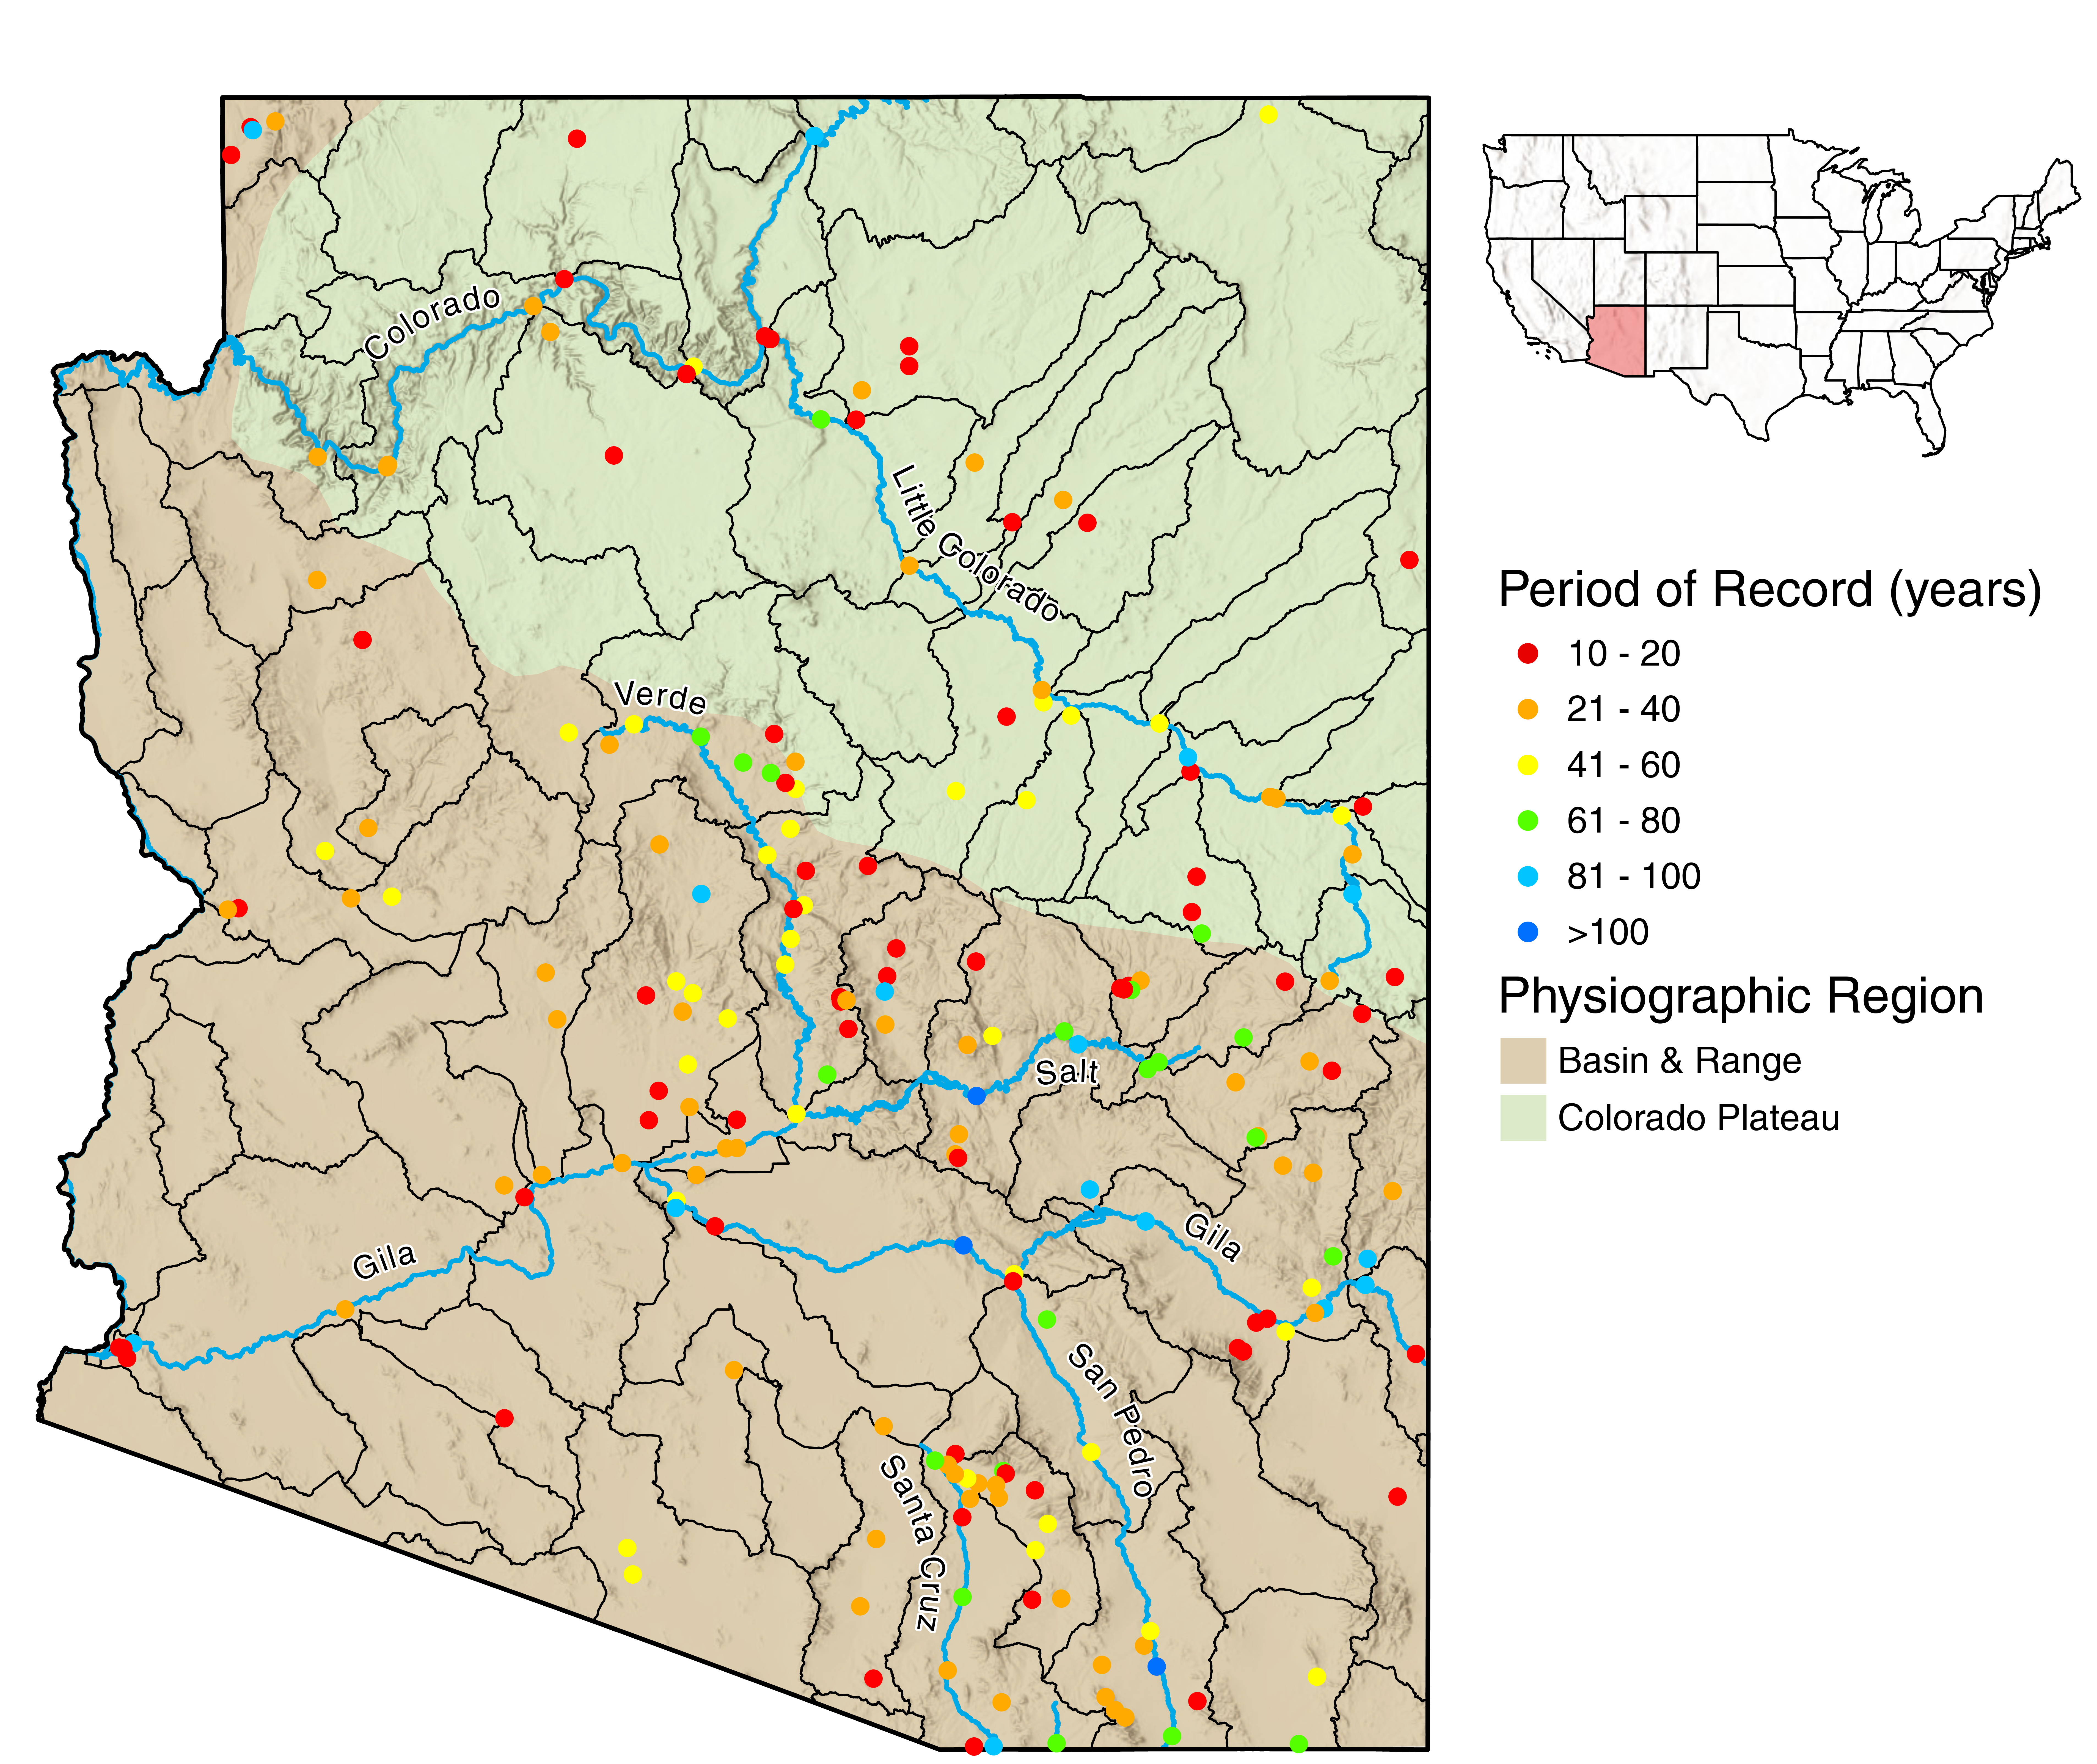
\includegraphics{images/StudyArea_20241203.png}

}

\caption{\label{fig-study-area}Map of Arizona indicating US Geological
Survey (USGS) streamgages used in this study. 8-digit HUC subbasin
boundaries and physiographic regions shown.}

\end{figure}%

Arizona's hydrology varies seasonally and spatially between its
physiographic regions. In the summer, localized and intense convective
precipitation events are driven by the North American Monsoon, while in
the winter, orographic precipitation comes from Pacific frontal systems
(Eastoe et al., 2019). While monsoonal precipitation can account for up
to 50\% of annual precipitation, evaporation and dry preceding soil
properties leads to most precipitation becoming runoff (Sheppard et al.,
2002). As such, 94\% of streams in Arizona are ephemeral or intermittent
(Levick et al., 2008). Much of the hydrology of Arizona is snow-melt
derived, driven by spring melt from the high-elevation Colorado Plateau
winter snowpack. While winter precipitation provides only 30\% of annual
averages, it provides the majority of water for natural reservoirs
(Sheppard et al., 2002).

\subsection{Data}\label{sec-data}

Daily observed streamflow data obtained from the United States
Geological Survey (USGS) National Water Information System (NWIS) were
used in this study. Streamgages were selected depending on criteria to
ensure the applicability of each site. O'Donnell et al. (2016) found
that 8-10 years of calibration data were necessary to account for
climate variability in paired watershed studies in the region. Following
this criteria, a minimum of 10 years of record was chosen. Any years
missing more than 30 days of streamflow were removed from the possible
record period. This analysis focuses on natural, streamflow-influencing
recharge, excluding streamgages affected by regulation or diversions.
These gages were identified through annual reports on water data
published by the USGS (USGS, 2010). Finally, streamgages on the Colorado
River were excluded from the dataset on the basis that they represent
managed flows shared by Colorado River Compact states. Following these
parameters, 205 USGS streamgages with acceptable periods of record were
used in this study (Figure~\ref{fig-study-area}). Periods of record
ranged from 10 to 112 years, with a median of 28 years.

Watersheds across the United States are delineated by the USGS using a
hydrologically-defined network. This system delineates the country using
hierarchical hydrologic unit codes (HUCs), where each subsequent basin
includes the digits of the enclosing basin. Here, 8-digit HUCs (HUC 8s)
are used to divide Arizona into 84 sub-basins that are fully or
partially in the state (Figure~\ref{fig-study-area}). These HUC 8
sub-basins are analogous to medium-sized river basins and are defined by
surface water characteristics.

Annual precipitation and temperature data came from the PRISM climate
group at Oregon State University at a resolution of 4 km
(\url{https://prism.oregonstate.edu;} (Daly et al., 2008)). The PRISM
dataset provides valuable insights into regional climate in ungauged
regions and has been shown to perform well across the southwestern US
(Buban et al., 2020)\textbf{.} Instead of the water year, PRISM data
uses a calendar-year format, which was adopted for consistency in the
water balance. Although this may introduce challenges in the annual
estimates due to inter-annual snow storage, the use of long-term annual
averages is likely to reduce any potential errors (Reitz et al., 2017).

Annual evapotranspiration (ET) data came from TerraClimate, a 4-km grid
climatalogical data set (Abatzoglou et al., 2018). TerraClimate uses a
Penman-Monteith approach to generate a reference potential
evapotranspiration (PET). The PET values were calculated assuming a
reference grass surface across the landscape with unlimited water. In
the drylands of the southwestern US, PET typically exceeds precipitation
annually (Zomer et al., 2022).

A 30-meter resolution Digital Elevation Model (DEM) of Arizona was used
to derive key basin characteristics: basin area, average slope, and the
proportion of each basin oriented toward north or south aspects. Various
geospatial variables, such as aspect, were disaggregated then averaged
to assess the areal percentage of each sub-variable within individual
HUC 8 basins. By calculating these percentages, we aimed to get a more
comprehensive understanding of landscape composition across space. Land
cover from USGS-NLCD (National Land Cover Database), hydrologic soil
group from SSURGO (Soil Survey Geographic Database), and underlying
geology and karst from USGS were all similarly averaged across the
basins. Aggregating variables to align with the HUC 8 boundaries allowed
for more precise predictions of BFI by integrating spatial variations
within each basin.

\subsection{Base-flow separation}\label{sec-bf_sep}

Directly measuring base flow and BFI presents unique challenges
(Eckhardt, 2008). The technique chosen to separate base flow has been
shown to affect results, and the choice of base-flow separation method
is subjective since `true' BFI values are not known (Beck et al., 2013).
However, many methods have been developed to estimate these values.
These methods include the use of tracers (Gonzales et al., 2009),
graphical interpolation (Institute of Hydrology, 1980; Sloto et al.,
1996), and digital filters (Arnold et al., 1995; Eckhardt, 2005; Lyne et
al., 1979; Nathan et al., 1990). These techniques have varying levels of
applicability depending on the spatial scale, time span, and the scope
of the study. Comparisons of various base-flow separation techniques
have been made in (Eckhardt, 2005, 2008; Nathan et al., 1990) , but this
study does not explore the superiority of different methods.

Base flow was calculated using a single-parameter, recursive digital
filter technique from (Nathan et al., 1990). This base-flow separation
technique is based on a recursive digital filter used in signal analysis
that separates high-frequency signals (quickflow) from low-frequency
signals (base flow) (Lyne et al., 1979). Eckhardt (2023) noted that
recursive digital filters lack a physical basis, but as the method is
easy to automate, objective, and repeatable, it is appropriate for a
regional-scale study. The Lyne-Hollick filter has been used in (Arnold
et al., 2000; Bloomfield et al., 2009; Santhi et al., 2008; Singh et
al., 2018). It takes the form of

\begin{equation}\phantomsection\label{eq-bf-separate}{
b = \alpha b_{k-1} + \frac{1-\alpha}{2}(Q_k + Q_{k-1})
}\end{equation}

where \(b\) is base flow, \(\alpha\) is the filter parameter, \(Q\) is
the total streamflow, and \(k\) is the time step. A filter parameter
\(\alpha\) of 0.925 was used as in Nathan et al. (1990) and Fuka et al.
(2014). The filter was run three times (forward, backward, forward) to
attenuate the base-flow signal.

\subsection{Machine Learning}\label{machine-learning}

The implementation of machine learning models to predict hydrologic
indices has been successful in past studies (Rozos et al., 2021; Schmidt
et al., 2020; Singh et al., 2018). In this work, we used the eXtreme
Gradient Boosting (XGBoost) algorithm (Chen et al., 2016) to predict BFI
at ungauged locations using catchment characteristics as predictors. The
XGBoost algorithm is a decision tree-based ensemble algorithm, which can
be adapted for either regression or classification problems. It has
grown in popularity in recent years due to its rapid, efficient, and
scalable nature, and has proven effective in similar environmental
modeling tasks such as streamflow forecasting Ni et al. (2020) and
classifying land use/land cover data (Georganos et al., 2018).

XGBoost uses gradient boosting on decision tree algorithms to leverage
the combination of multiple very low variance models into one overall
prediction. Gradient boosting works sequentially, with the first tree
being learned on the known target values, and each subsequent tree being
learned on the errors of the tree prior. The algorithm then applies a
weighting to each tree based on this boosting to determine how much the
tree will contribute towards the final output. The final prediction is
obtained by the input data traversing all \(n\) weighted trees in the
learned ensemble. The trained XGBoost model is used to predict BFI in
ungauged catchments based on geospatial and hydroclimate predictor
variables (Table~\ref{tbl-predictors}). Certain features were subdivided
according to their areal coverage of each basin (e.g.~land cover was
divided into 16 subdivisions).

\begin{longtable}[]{@{}
  >{\raggedright\arraybackslash}p{(\columnwidth - 6\tabcolsep) * \real{0.2329}}
  >{\raggedright\arraybackslash}p{(\columnwidth - 6\tabcolsep) * \real{0.2877}}
  >{\raggedright\arraybackslash}p{(\columnwidth - 6\tabcolsep) * \real{0.2329}}
  >{\raggedright\arraybackslash}p{(\columnwidth - 6\tabcolsep) * \real{0.2466}}@{}}
\caption{Basin-characteristic variables used as initial features in
XGBoost model. Starred features are maintained in the final,
dimensionality-reduced model.}\label{tbl-predictors}\tabularnewline
\toprule\noalign{}
\begin{minipage}[b]{\linewidth}\raggedright
\end{minipage} & \begin{minipage}[b]{\linewidth}\raggedright
Variable
\end{minipage} & \begin{minipage}[b]{\linewidth}\raggedright
Source
\end{minipage} & \begin{minipage}[b]{\linewidth}\raggedright
Geoprocessing
\end{minipage} \\
\midrule\noalign{}
\endfirsthead
\toprule\noalign{}
\begin{minipage}[b]{\linewidth}\raggedright
\end{minipage} & \begin{minipage}[b]{\linewidth}\raggedright
Variable
\end{minipage} & \begin{minipage}[b]{\linewidth}\raggedright
Source
\end{minipage} & \begin{minipage}[b]{\linewidth}\raggedright
Geoprocessing
\end{minipage} \\
\midrule\noalign{}
\endhead
\bottomrule\noalign{}
\endlastfoot
Hydroclimate & Precipitation* & PRISM & Basin average \\
& Mean Temperature* & PRISM & Basin average \\
& Mean Evapotranspiration* & TerraClimate & Basin average \\
Geospatial & Elevation* & DEM & Basin average \\
& Area & DEM & Basin average \\
& Slope & DEM & Basin average \\
& Aspect & DEM & Percent areal coverage \\
& Land Cover* & NLCD & Percent areal coverage \\
& Hydrologic Soil Group* & SSURGO & Percent areal coverage \\
& Geology & USGS & Percent areal coverage \\
& Karst & USGS & Percent areal coverage \\
\end{longtable}

\subsubsection{Feature Selection}\label{feature-selection}

Machine learning models can face issues with overfitting when provided
with a large set of predicting features. This can cause reductions in
performance on unseen data and requires greater computational power and
memory storage (Li et al., 2017). Dimensionality reduction is a powerful
tool in addressing these issues which can be divided into two broad
categories: feature extraction and feature selection. Feature extraction
involves projecting the higher dimensional dataset to a feature space
with less dimensions, though this entails creating a new set of features
that lose the physical meaning of the original feature space. On the
other hand, feature selection maintains a subset of the original
features, all of which retain their physical meaning providing better
readability and interpretability. Here, a supervised features selection
was used to reduce the number of predictors and, as a result, increased
learning performance, decreased computational costs, and reduced
overfitting.

An initial model was trained on the full feature set of 45 predictors
(Table~\ref{tbl-predictors}). We then used a feature importance method
of feature selection to remove noise and less-important features.
Feature importance scores are an approach where importance scores are
assigned to individual features indicating how much the feature
contributed (positively or negatively) to the model (Murdoch et al.,
2019). Here, we use SHAP (SHapley Additive exPlanations) values as the
method of assigning importance values to each feature (Lundberg \& Lee,
2017). The top-10 most-important features
(\textbf{?@suppfig-shap\_values}) were subset and used in training a
subsequent model which saw performance increases and reduced computing
time. This subsequent model was used as the final model in this
analysis.

\subsection{Statistical Analyses}\label{statistical-analyses}

Statisical analyses were performed on annual BFI and base flow values of
instrumented streamgages. We examined temporal trends using the
Mann-Kendall nonparametric trend test to determine the presence of
monotonic trends (Kendall, 1970; Mann, 1945). The Mann-Kendall test was
used to determine trends in BFI and trend significance of gauged
reaches. This test is widely used in studies of this kind (Ayers et al.,
2019; Ficklin et al., 2016; Woodhouse et al., 2022).

Trends in BFI and base flow were produced using a Mann-Kendall test for
monotonic trends. This test expects that the data is non-parametric and
that the observations are not autocorrelated over time. Observations at
4 streamgages show significant autocorrelation, though only one
streamgage (09486500 - Santa Cruz River at Cortaro, AZ) indicated a
significant trend in BFI. Due to this autocorrelation, the streamgage
was removed from the trend analysis as the autocorrelation may inflate
the variance of the Mann-Kendall statistic leading to an
over/underestimate of the trend (Hamed \& Rao, 1998).

Trends with a \(\rho \le 0.05\) are considered significant.

\section{Results}\label{results}

\subsection{BFI of Gauged Catchments}\label{bfi-of-gauged-catchments}

\begin{figure}

\centering{

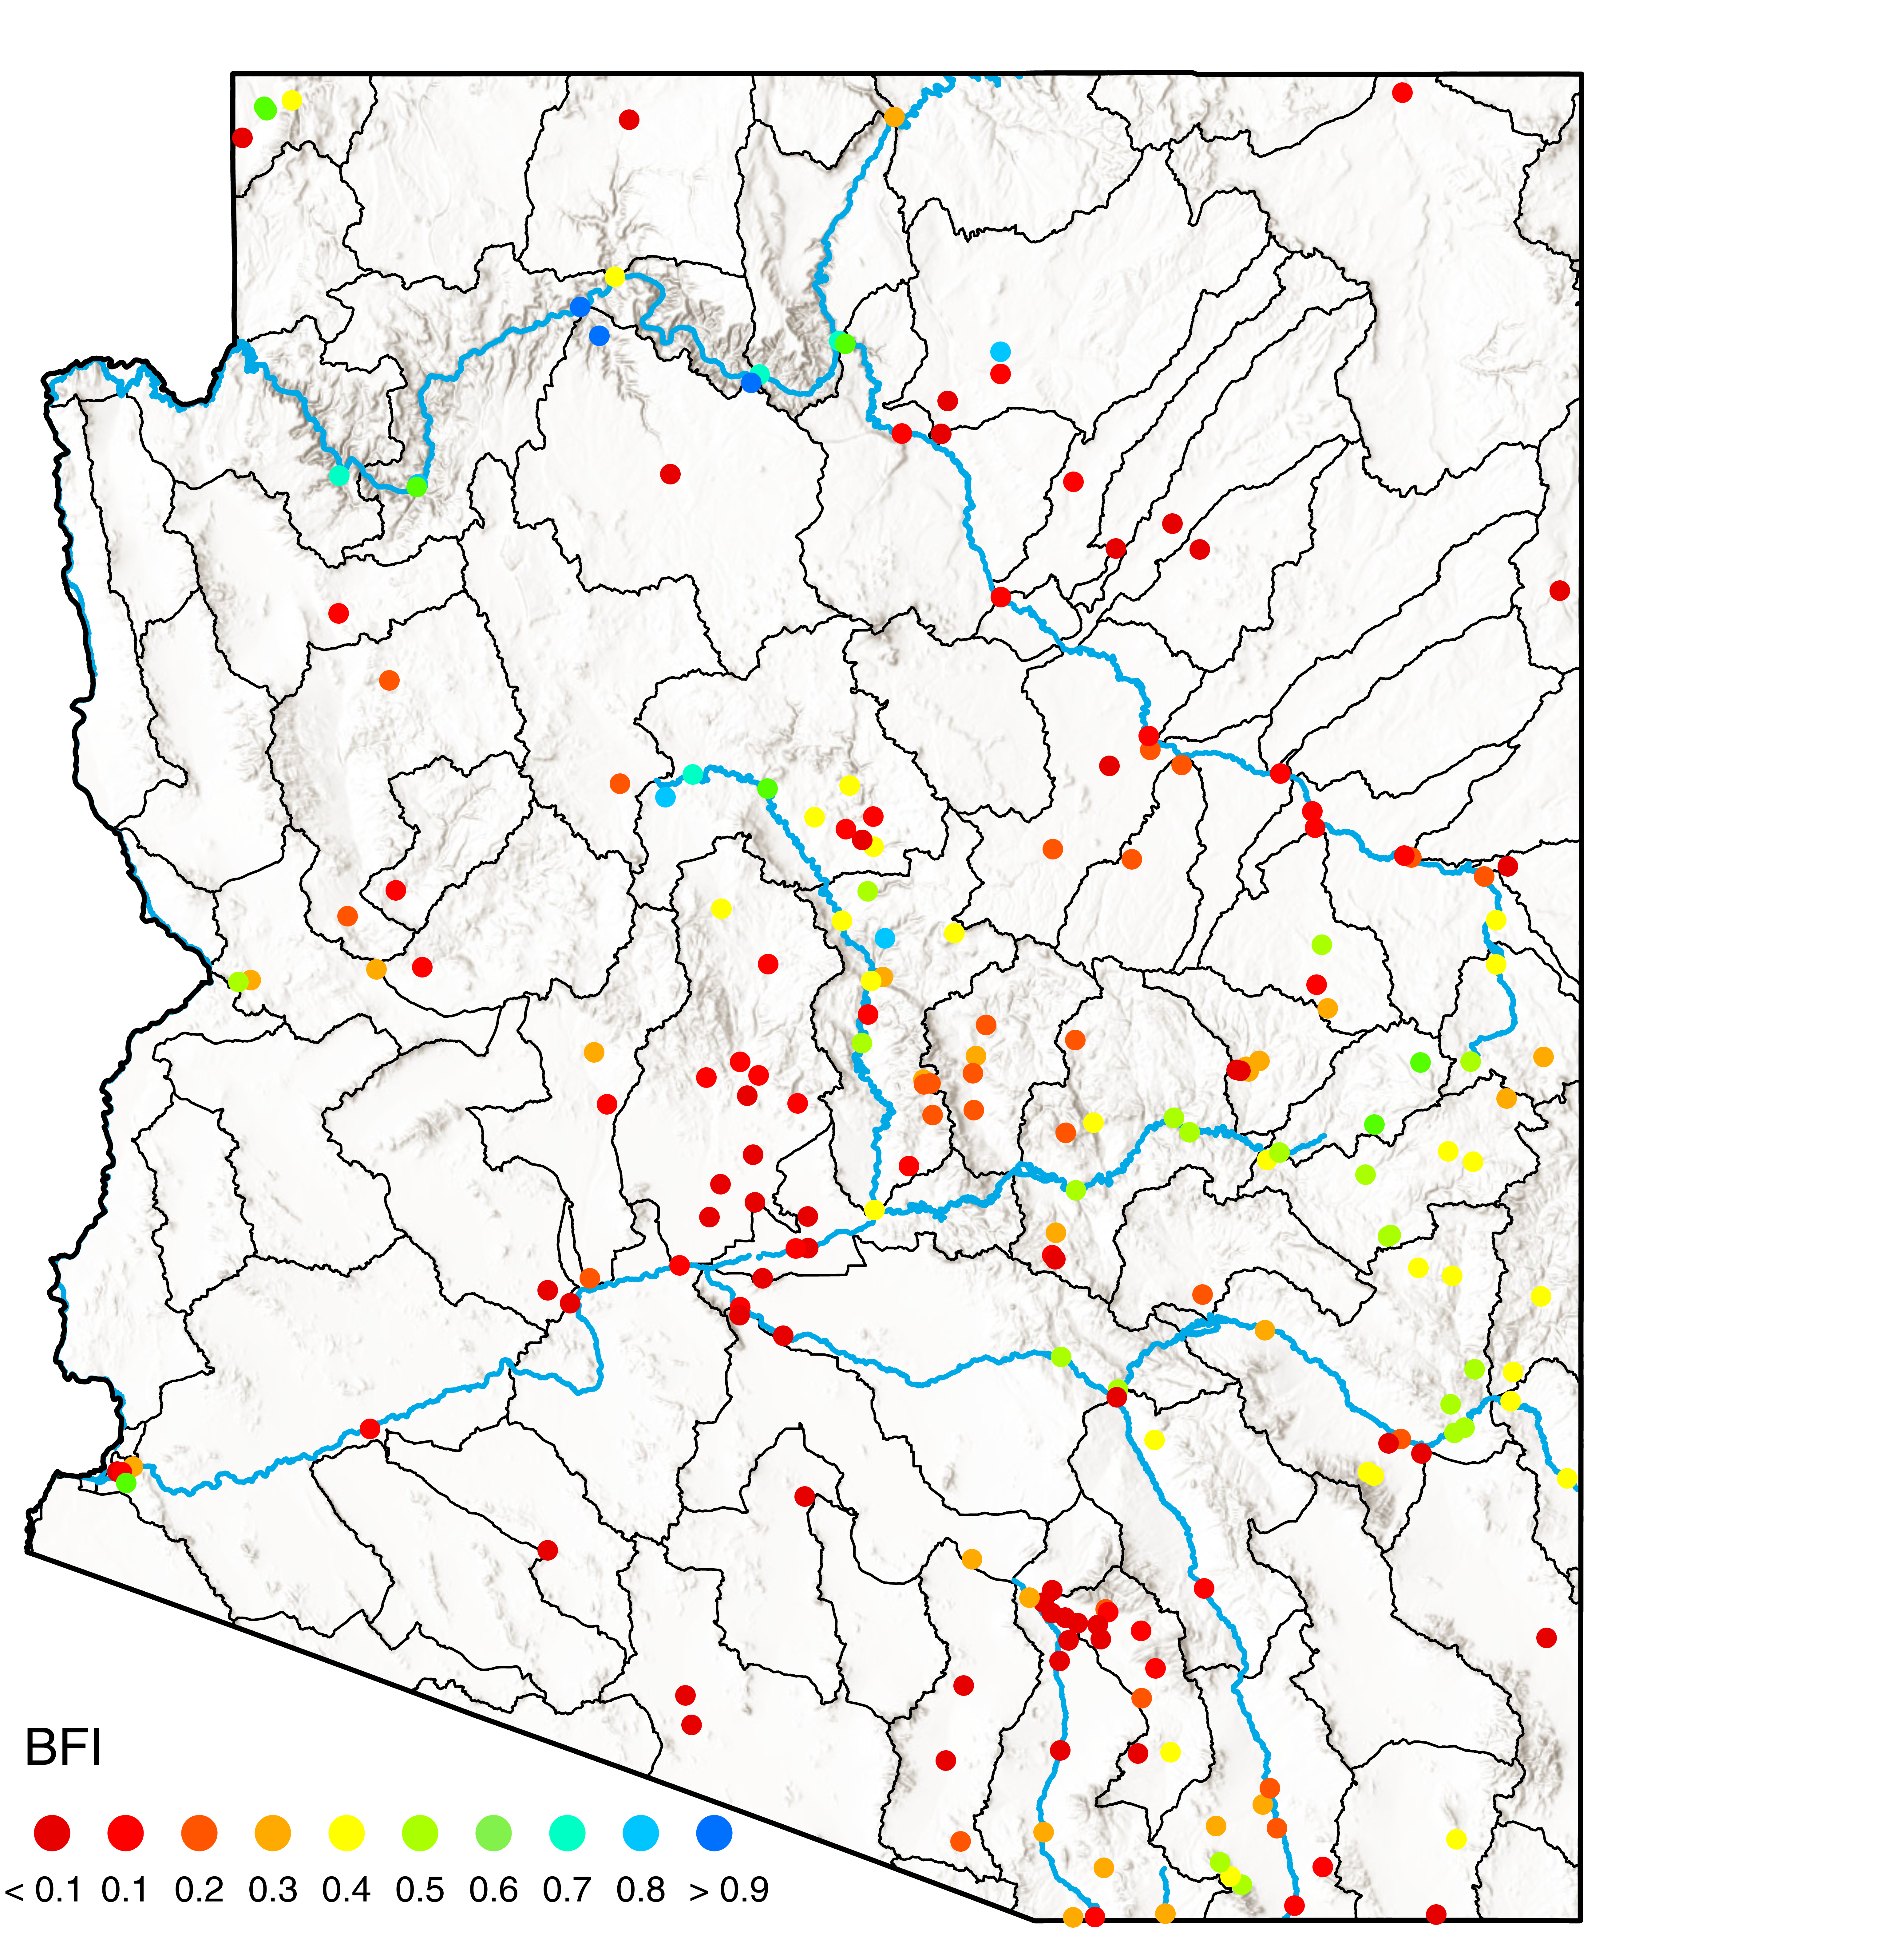
\includegraphics{images/BFI_Instrumented_20241203.png}

}

\caption{\label{fig-instrumented-bfi}Mean annual BFI for the period of
record from instrumented stream flow data.}

\end{figure}%

The long-term average BFI for the 205 gauged reaches across Arizona is
illustrated in Figure~\ref{fig-instrumented-bfi} . The highest BFI
values (\textgreater0.9) are found along the Grand Canyon in
northwestern Arizona. The highly karstic geology of this region
facilitates the rapid movement of subsurface flow to surface water and
spring outlets (Chambless et al., 2023). Relatively high BFI values
(\textgreater0.8) are found at the spring-fed headwaters of the Verde
River (Del Rio Spring) and the spring-fed headwaters of Fossil Creek.
These results are consistent with interpolated BFI values reported by
Wolock (2003).

The stream reaches of the Little Colorado River Basin (northeastern
Arizona) indicate consisently low BFI values (\textless{} 0.2). This is
likely due to low-yielding perched aquifers underlying the Defiance
Uplift in northeastern Arizona, which are hydrologically connected to
surface streams, while the high-yield, confined regional aquifer is much
deeper (Blanchard, 2002). This region also typifies a pattern of seen
along most major rivers in the study area: upstream reaches indicate
higher BFI values while the downstream reaches display lower BFI values.
This is assumed to be due to greater groundwater-surface water
interaction at the headwaters of streams (likely due to spring outlets)
and the dilution of base flow while moving down stream
(\textbf{CITATION}). This pattern is seen along the Gila River, Verde
River, and Little Colorado Rivers in Arizona.

\subsubsection{Trends in BFI}\label{sec-bfi-trends}

Trends in BFI over the period of record for each streamgage in this
analysis are illustrated in Figure~\ref{fig-instrumented-trend} and
Table~\ref{tbl-trends} .

\begin{figure}

\centering{

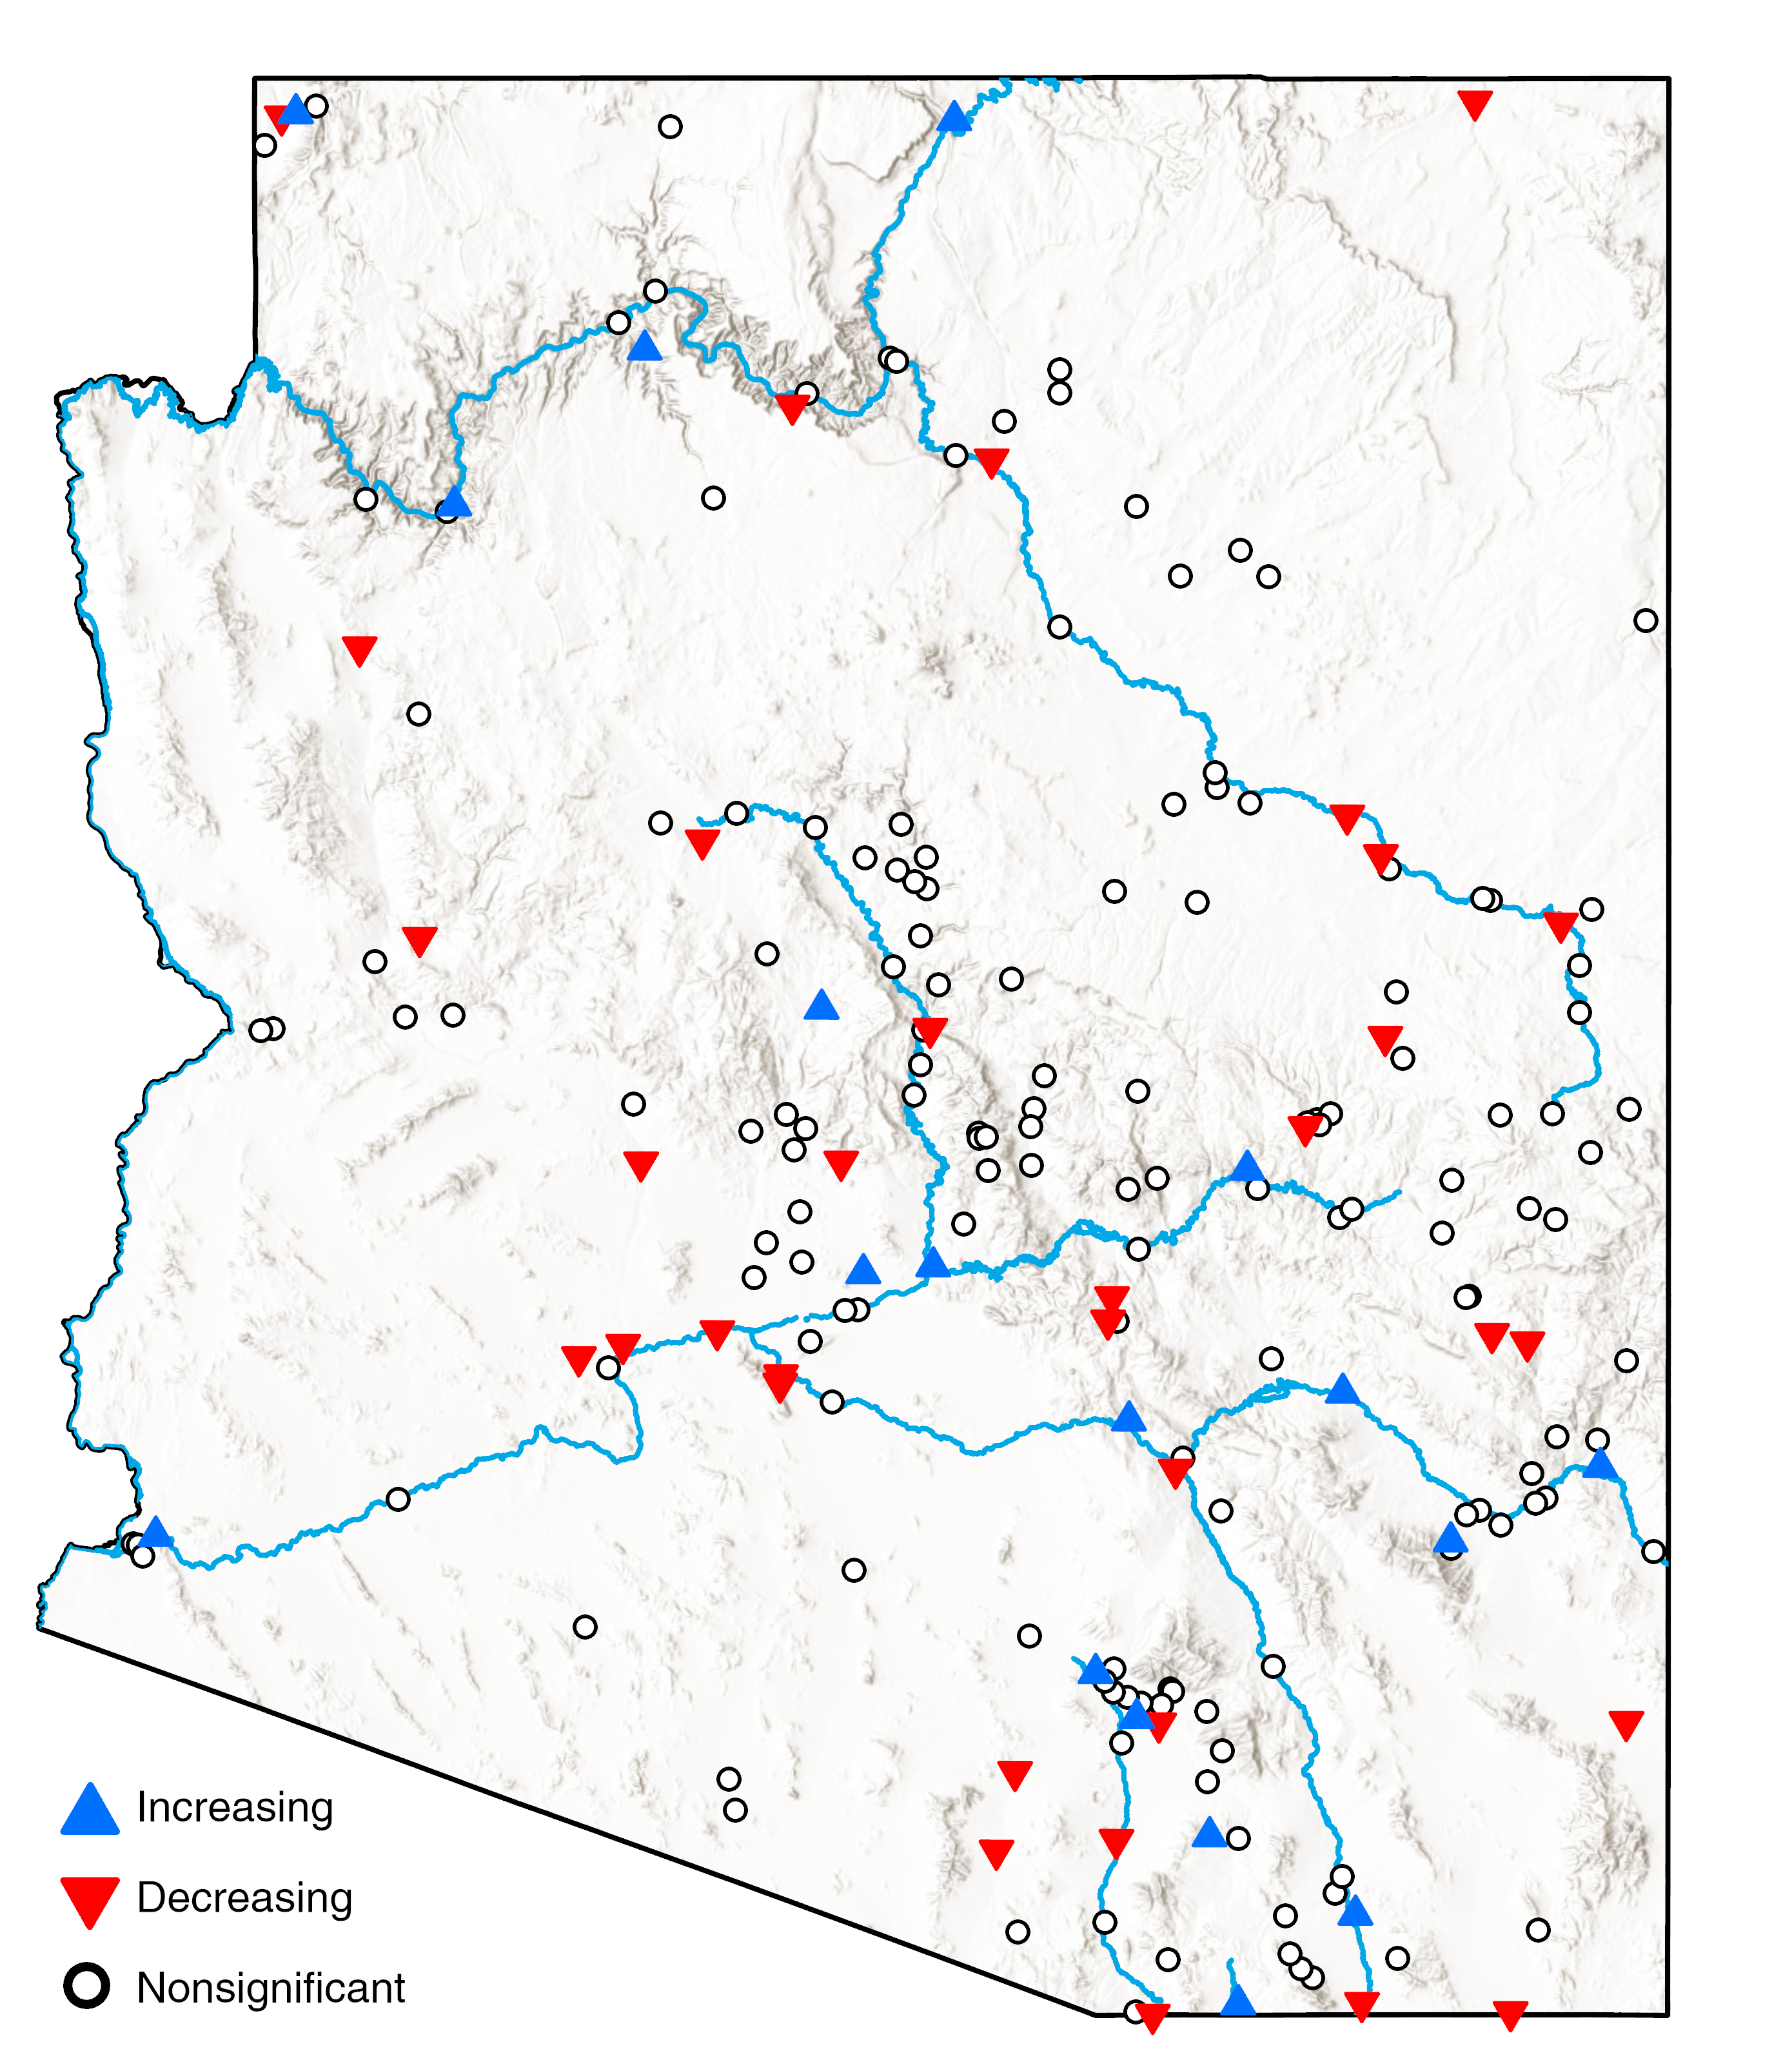
\includegraphics{images/BFITrends_20241203.png}

}

\caption{\label{fig-instrumented-trend}Trends in BFI over full period of
record for instrumented sites used in this study. Red upward (blue
downward) arrows indicate an increasing (decreasing) trend at a
significance level of 5\%. White circles represent sites with no
statistically significant trends.}

\end{figure}%

\begin{longtable}[]{@{}
  >{\raggedright\arraybackslash}p{(\columnwidth - 10\tabcolsep) * \real{0.4800}}
  >{\raggedright\arraybackslash}p{(\columnwidth - 10\tabcolsep) * \real{0.0667}}
  >{\raggedright\arraybackslash}p{(\columnwidth - 10\tabcolsep) * \real{0.0933}}
  >{\raggedright\arraybackslash}p{(\columnwidth - 10\tabcolsep) * \real{0.0933}}
  >{\raggedright\arraybackslash}p{(\columnwidth - 10\tabcolsep) * \real{0.1333}}
  >{\raggedright\arraybackslash}p{(\columnwidth - 10\tabcolsep) * \real{0.1333}}@{}}
\caption{Comparison of trends for BFI for all sites split by various
classifications. Only sites with a significant (\(\rho \le 0.05\)) trend
are included here as established by a Mann-Kendall test for monotonic
trends across the full period of record. n is the number of sites,
n\_pos (n\_neg) is the number of sites with positive (negative) trends,
perc\_pos (perc\_neg) is the percentage of n with a positive (negative)
trend.}\label{tbl-trends}\tabularnewline
\toprule\noalign{}
\begin{minipage}[b]{\linewidth}\raggedright
Classification Group
\end{minipage} & \begin{minipage}[b]{\linewidth}\raggedright
n
\end{minipage} & \begin{minipage}[b]{\linewidth}\raggedright
n\_pos
\end{minipage} & \begin{minipage}[b]{\linewidth}\raggedright
n\_neg
\end{minipage} & \begin{minipage}[b]{\linewidth}\raggedright
perc\_pos
\end{minipage} & \begin{minipage}[b]{\linewidth}\raggedright
perc\_neg
\end{minipage} \\
\midrule\noalign{}
\endfirsthead
\toprule\noalign{}
\begin{minipage}[b]{\linewidth}\raggedright
Classification Group
\end{minipage} & \begin{minipage}[b]{\linewidth}\raggedright
n
\end{minipage} & \begin{minipage}[b]{\linewidth}\raggedright
n\_pos
\end{minipage} & \begin{minipage}[b]{\linewidth}\raggedright
n\_neg
\end{minipage} & \begin{minipage}[b]{\linewidth}\raggedright
perc\_pos
\end{minipage} & \begin{minipage}[b]{\linewidth}\raggedright
perc\_neg
\end{minipage} \\
\midrule\noalign{}
\endhead
\bottomrule\noalign{}
\endlastfoot
Precipitation - Monsoon Dominated & 87 & 8 & 21 & 0.092 & 0.241 \\
Precipitation - Snowmelt Dominated & 118 & 9 & 12 & 0.076 & 0.102 \\
PhysRegion - Basin\&Range & 156 & 14 & 26 & 0.090 & 0.167 \\
PhysRegion - CO Plateau & 49 & 3 & 7 & 0.061 & 0.143 \\
Climate - Warm-Wet & 31 & 2 & 6 & 0.065 & 0.194 \\
Climate - Warm-Dry & 55 & 6 & 11 & 0.109 & 0.200 \\
Climate - Cool-Wet & 74 & 4 & 9 & 0.054 & 0.122 \\
Climate - Cool-Dry & 45 & 5 & 7 & 0.111 & 0.156 \\
Slope - High & 102 & 10 & 12 & 0.098 & 0.118 \\
Slope - Low & 103 & 7 & 21 & 0.068 & 0.204 \\
\end{longtable}

\subsection{BFI of Ungauged
Catchments}\label{bfi-of-ungauged-catchments}

\subsubsection{Predictor Importance}\label{predictor-importance}

\begin{figure}

\centering{

\includegraphics{images/actual-predicted.png}

}

\caption{\label{fig-actual_predicted}Linear relationship between
observed BFI and predicted BFI. The solid line is the 1:1 line, the
dashed line is regressed to the data.}

\end{figure}%

\subsubsection{Model Validation}\label{model-validation}

\begin{longtable}[]{@{}
  >{\raggedright\arraybackslash}p{(\columnwidth - 14\tabcolsep) * \real{0.3846}}
  >{\raggedright\arraybackslash}p{(\columnwidth - 14\tabcolsep) * \real{0.0769}}
  >{\raggedright\arraybackslash}p{(\columnwidth - 14\tabcolsep) * \real{0.0897}}
  >{\raggedright\arraybackslash}p{(\columnwidth - 14\tabcolsep) * \real{0.0897}}
  >{\raggedright\arraybackslash}p{(\columnwidth - 14\tabcolsep) * \real{0.0897}}
  >{\raggedright\arraybackslash}p{(\columnwidth - 14\tabcolsep) * \real{0.0897}}
  >{\raggedright\arraybackslash}p{(\columnwidth - 14\tabcolsep) * \real{0.0897}}
  >{\raggedright\arraybackslash}p{(\columnwidth - 14\tabcolsep) * \real{0.0897}}@{}}
\caption{Performance of model predictions for BFI for all sites split by
various classifications. n is number of observatios,
R\textsuperscript{2} is the coefficient of determination of a linear
regression, MSE is mean-squared-error, RMSE is root-mean-squared-error,
MAE is mean-absolute-error, NSE is Nash-Sucliffe efficiency, and pbias
is percent bias.}\label{tbl-performance}\tabularnewline
\toprule\noalign{}
\begin{minipage}[b]{\linewidth}\raggedright
Classification Group
\end{minipage} & \begin{minipage}[b]{\linewidth}\raggedright
n
\end{minipage} & \begin{minipage}[b]{\linewidth}\raggedright
R2
\end{minipage} & \begin{minipage}[b]{\linewidth}\raggedright
MSE
\end{minipage} & \begin{minipage}[b]{\linewidth}\raggedright
RMSE
\end{minipage} & \begin{minipage}[b]{\linewidth}\raggedright
MAE
\end{minipage} & \begin{minipage}[b]{\linewidth}\raggedright
NSE
\end{minipage} & \begin{minipage}[b]{\linewidth}\raggedright
pbias
\end{minipage} \\
\midrule\noalign{}
\endfirsthead
\toprule\noalign{}
\begin{minipage}[b]{\linewidth}\raggedright
Classification Group
\end{minipage} & \begin{minipage}[b]{\linewidth}\raggedright
n
\end{minipage} & \begin{minipage}[b]{\linewidth}\raggedright
R2
\end{minipage} & \begin{minipage}[b]{\linewidth}\raggedright
MSE
\end{minipage} & \begin{minipage}[b]{\linewidth}\raggedright
RMSE
\end{minipage} & \begin{minipage}[b]{\linewidth}\raggedright
MAE
\end{minipage} & \begin{minipage}[b]{\linewidth}\raggedright
NSE
\end{minipage} & \begin{minipage}[b]{\linewidth}\raggedright
pbias
\end{minipage} \\
\midrule\noalign{}
\endhead
\bottomrule\noalign{}
\endlastfoot
Climate - Monsoon Dominated & 3039 & 0.633 & 0.016 & 0.126 & 0.074 &
0.619 & -13.7 \\
Climate - Snowmelt Dominated & 4685 & 0.733 & 0.015 & 0.121 & 0.087 &
0.725 & -3.5 \\
PhysRegion - Basin\&Range & 6147 & 0.733 & 0.016 & 0.127 & 0.084 & 0.724
& -6.3 \\
PhysRegion - CO Plateau & 1577 & 0.846 & 0.011 & 0.104 & 0.073 & 0.843 &
-3.8 \\
Climate - Warm-Wet & 1506 & 0.693 & 0.014 & 0.117 & 0.077 & 0.685 &
-8.2 \\
Climate - Warm-Dry & 2351 & 0.693 & 0.022 & 0.147 & 0.092 & 0.675 &
-11.9 \\
Climate - Cool-Wet & 2350 & 0.738 & 0.011 & 0.106 & 0.078 & 0.736 &
-1.7 \\
Climate - Cool-Dry & 1517 & 0.831 & 0.012 & 0.111 & 0.078 & 0.827 &
-4.3 \\
Slope - High & 3795 & 0.776 & 0.012 & 0.111 & 0.079 & 0.771 & -3.3 \\
Slope - Low & 3929 & 0.724 & 0.018 & 0.133 & 0.085 & 0.713 & -9.1 \\
\end{longtable}

Consistently negative pbias values across all classifications suggest an
under-prediction of BFI.

\subsubsection{Predictor Importance}\label{sec-predictor-importance}

\subsubsection{Predicted Long-term Mean
BFI}\label{predicted-long-term-mean-bfi}

\begin{figure}

\centering{

\includegraphics{images/BFI_HUC8_20241203.png}

}

\caption{\label{fig-bfi-huc}Predicted mean annual BFI values for 8-digit
HUC (1991-2020)}

\end{figure}%

\begin{figure}

\centering{

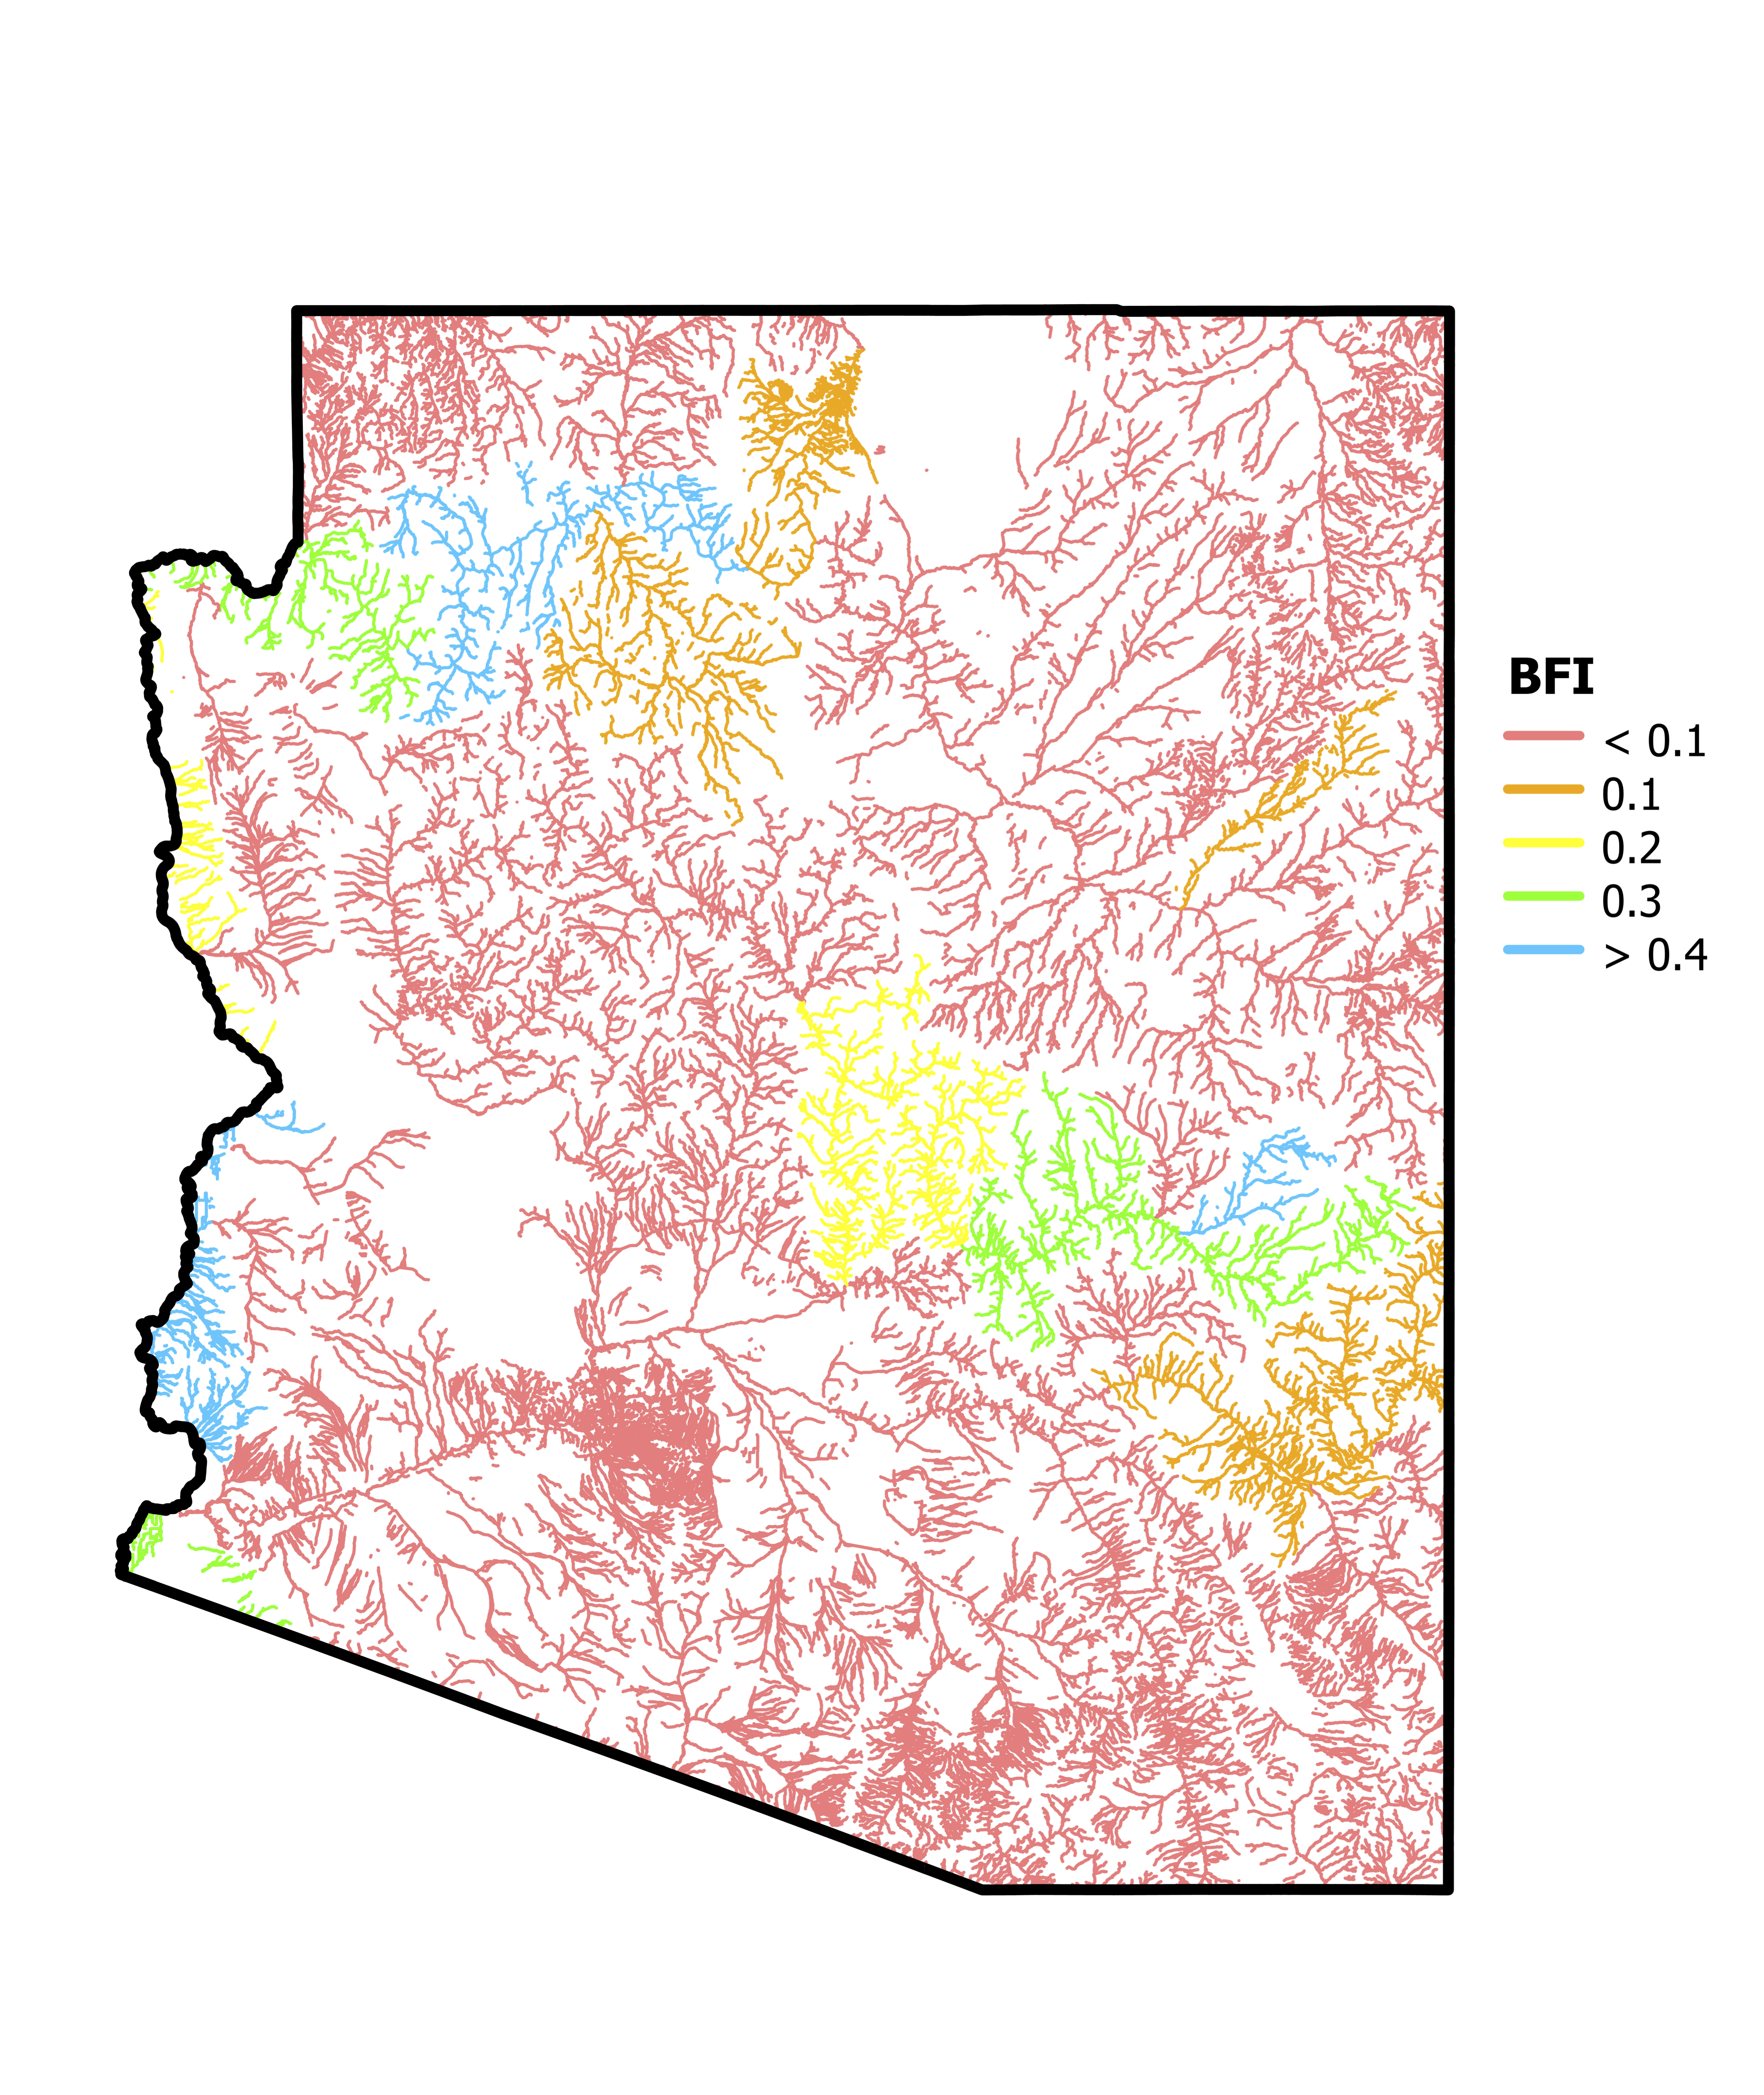
\includegraphics{images/BFI_AllStream.png}

}

\caption{\label{fig-bfi-streams}Predicted mean annual BFI values for all
reaches of Strahler stream order 3 and greater}

\end{figure}%

\section{Conclusion}\label{sec-conclusion}

\section*{References}\label{references}
\addcontentsline{toc}{section}{References}

\section{Supporting Information}\label{supporting-information}

\includegraphics{images/supplemental/shap_summary.png}
\{\#suppfig-shap\_values\}

\phantomsection\label{refs}
\begin{CSLReferences}{1}{0}
\bibitem[\citeproctext]{ref-abatzoglou2018}
Abatzoglou, J. T. et al. (2018). TerraClimate, a high-resolution global
dataset of monthly climate and climatic water balance from
1958{\textendash}2015. \emph{Scientific Data}, \emph{5}(1), 170191.
\url{https://doi.org/10.1038/sdata.2017.191}

\bibitem[\citeproctext]{ref-ahiablame2013}
Ahiablame, L. et al. (2013). Estimation of annual baseflow at ungauged
sites in Indiana USA. \emph{Journal of Hydrology}, \emph{476}, 13--27.
\url{https://doi.org/10.1016/j.jhydrol.2012.10.002}

\bibitem[\citeproctext]{ref-arnold1995}
Arnold, J. G. et al. (1995). Automated Base Flow Separation and
Recession Analysis Techniques. \emph{Ground Water}, \emph{33}(6),
1010--1018. \url{https://doi.org/10.1111/j.1745-6584.1995.tb00046.x}

\bibitem[\citeproctext]{ref-ARNOLD200021}
Arnold, J. G. et al. (2000). Regional estimation of base flow and
groundwater recharge in the upper mississippi river basin. \emph{Journal
of Hydrology}, \emph{227}(1), 21--40.
https://doi.org/\url{https://doi.org/10.1016/S0022-1694(99)00139-0}

\bibitem[\citeproctext]{ref-ayers2019}
Ayers, J. R., Villarini, G., Jones, C., \& Schilling, K. (2019). Changes
in monthly baseflow across the U.S. Midwest. \emph{Hydrological
Processes}, \emph{33}(5), 748--758.
\url{https://doi.org/10.1002/hyp.13359}

\bibitem[\citeproctext]{ref-beck2013}
Beck, H. E. et al. (2013). Global patterns in base flow index and
recession based on streamflow observations from 3394 catchments: Global
Patterns in Base Flow Characteristics. \emph{Water Resources Research},
\emph{49}(12), 7843--7863. \url{https://doi.org/10.1002/2013WR013918}

\bibitem[\citeproctext]{ref-blanchard02}
Blanchard, P. J. (2002). \emph{Assessments of aquifer sensitivity on
{Navajo Nation} and adjacent lands and ground-water vulnerability to
pesticide contamination on the {Navajo Indian Irrigation Project},
{Arizona}, {New Mexico}, and {Utah}} (No. Water-Resources Investigations
Report 02-4051). {USGS}. \url{https://doi.org/10.3133/wri024051}

\bibitem[\citeproctext]{ref-bloomfield2009}
Bloomfield, J. P. et al. (2009). Examining geological controls on
baseflow index (BFI) using regression analysis: An illustration from the
Thames Basin, UK. \emph{Journal of Hydrology}, \emph{373}(1-2),
164--176. \url{https://doi.org/10.1016/j.jhydrol.2009.04.025}

\bibitem[\citeproctext]{ref-bosch2017}
Bosch, D. D. et al. (2017). Temporal variations in baseflow for the
Little River experimental watershed in South Georgia, USA. \emph{Journal
of Hydrology: Regional Studies}, \emph{10}, 110--121.
\url{https://doi.org/10.1016/j.ejrh.2017.02.002}

\bibitem[\citeproctext]{ref-buban_PRISM}
Buban, M. S. et al. (2020). A comparison of the u.s. Climate reference
network precipitation data to the parameter-elevation regressions on
independent slopes model (PRISM). \emph{Journal of Hydrometeorology},
\emph{21}(10), 2391--2400. \url{https://doi.org/10.1175/JHM-D-19-0232.1}

\bibitem[\citeproctext]{ref-chambless_deep-karst_2023}
Chambless, H. E. et al. (2023). Deep-karst aquifer spring-flow trends in
a water-limited system, grand canyon national park, {USA}.
\emph{Hydrogeology Journal}, \emph{31}(7), 1755--1771.
\url{https://doi.org/10.1007/s10040-023-02702-w}

\bibitem[\citeproctext]{ref-chen2016xgboost}
Chen, T. et al. (2016). Xgboost: A scalable tree boosting system. In
\emph{Proceedings of the 22nd acm sigkdd international conference on
knowledge discovery and data mining} (pp. 785--794).

\bibitem[\citeproctext]{ref-daly2008}
Daly, C. et al. (2008). Physiographically sensitive mapping of
climatological temperature and precipitation across the conterminous
United States. \emph{International Journal of Climatology},
\emph{28}(15), 2031--2064. \url{https://doi.org/10.1002/joc.1688}

\bibitem[\citeproctext]{ref-eastoe2019mtnblock}
Eastoe, C. J. et al. (2019). Hydrology of mountain blocks in arizona and
new mexico as revealed by isotopes in groundwater and precipitation.
\emph{Geosciences}, \emph{9}(11).
\url{https://doi.org/10.3390/geosciences9110461}

\bibitem[\citeproctext]{ref-eckhardt2005}
Eckhardt, K. (2005). How to construct recursive digital filters for
baseflow separation. \emph{Hydrological Processes}, \emph{19}(2),
507--515. \url{https://doi.org/10.1002/hyp.5675}

\bibitem[\citeproctext]{ref-eckhardt2008}
Eckhardt, K. (2008). A comparison of baseflow indices, which were
calculated with seven different baseflow separation methods.
\emph{Journal of Hydrology}, \emph{352}(1-2), 168--173.
\url{https://doi.org/10.1016/j.jhydrol.2008.01.005}

\bibitem[\citeproctext]{ref-eckhardt2023}
Eckhardt, K. (2023). Technical note: How physically based is hydrograph
separation by recursive digital filtering? \emph{Hydrology and Earth
System Sciences}, \emph{27}(2), 495--499.
\url{https://doi.org/10.5194/hess-27-495-2023}

\bibitem[\citeproctext]{ref-fekete2007}
Fekete, B. M. et al. (2007). The current status of global river
discharge monitoring and potential new technologies complementing
traditional discharge measurements.

\bibitem[\citeproctext]{ref-ficklin2016}
Ficklin, D. L. et al. (2016). Impacts of recent climate change on trends
in baseflow and stormflow in United States watersheds. \emph{Geophysical
Research Letters}, \emph{43}(10), 5079--5088.
\url{https://doi.org/10.1002/2016GL069121}

\bibitem[\citeproctext]{ref-fuka2014ecohydrology}
Fuka, D. et al. (2014). EcoHydRology: A community modeling foundation
for eco-hydrology. \emph{R Package Version 0.4}, \emph{12}.

\bibitem[\citeproctext]{ref-Georganos2018Very}
Georganos, S. et al. (2018). Very high resolution object-based land
use--land cover urban classification using extreme gradient boosting.
\emph{IEEE Geoscience and Remote Sensing Letters}, \emph{15}, 607--611.
\url{https://doi.org/10.1109/LGRS.2018.2803259}

\bibitem[\citeproctext]{ref-gonzales2009}
Gonzales, A. L. et al. (2009). Comparison of different base flow
separation methods in a lowland catchment. \emph{Hydrology and Earth
System Sciences}, \emph{13}(11), 2055--2068.
\url{https://doi.org/10.5194/hess-13-2055-2009}

\bibitem[\citeproctext]{ref-MK_Hamed1998}
Hamed, K. H., \& Rao, A. (1998). A modified mann-kendall trend test for
autocorrelated data. \emph{Journal of Hydrology}, \emph{204}(1),
182--196.
https://doi.org/\url{https://doi.org/10.1016/S0022-1694(97)00125-X}

\bibitem[\citeproctext]{ref-instituteofhydrology1980}
Institute of Hydrology. (1980). \emph{Low flow studies report 3
catchment characteristic estimation manual}.

\bibitem[\citeproctext]{ref-iucn-drylands-2019}
IUCN. (2019, September). Drylands and climate change. Retrieved from
\url{https://www.iucn.org/resources/issues-brief/drylands-and-climate-change}

\bibitem[\citeproctext]{ref-kendall1970}
Kendall, M. G. (1970). \emph{Rank correlation methods} (4th ed). London:
Griffin.

\bibitem[\citeproctext]{ref-epa_AZephemeral}
Levick, L. R. et al. (2008). {The ecological and hydrological
significance of ephemeral and intermittent streams in the arid and
semi-arid American Southwest}. \emph{U.S. Environmental Protection
Agency and USDA/ARS Southwest Watershed Research Center},
(EPA/600/R-08/134).

\bibitem[\citeproctext]{ref-feat_selec2017}
Li, J., Cheng, K., Wang, S., Morstatter, F., Trevino, R. P., Tang, J.,
\& Liu, H. (2017). Feature selection: A data perspective. \emph{ACM
Comput. Surv.}, \emph{50}(6). \url{https://doi.org/10.1145/3136625}

\bibitem[\citeproctext]{ref-SHAP_values}
Lundberg, S. M., \& Lee, S.-I. (2017). A unified approach to
interpreting model predictions, \emph{30}. Retrieved from
\url{https://proceedings.neurips.cc/paper_files/paper/2017/file/8a20a8621978632d76c43dfd28b67767-Paper.pdf}

\bibitem[\citeproctext]{ref-lyne1979}
Lyne, V. et al. (1979). Institute of engineers australia national
conference. In (Vol. 79, pp. 89--93). Barton, Australia: Institute of
Engineers Australia.

\bibitem[\citeproctext]{ref-mann1945nonparametric}
Mann, H. B. (1945). Nonparametric tests against trend.
\emph{Econometrica: Journal of the Econometric Society}, 245--259.

\bibitem[\citeproctext]{ref-ML_interpretability2019}
Murdoch, W. J., Singh, C., Kumbier, K., Abbasi-Asl, R., \& Yu, B.
(2019). Definitions, methods, and applications in interpretable machine
learning. \emph{Proceedings of the National Academy of Sciences},
\emph{116}(44), 22071--22080.
\url{https://doi.org/10.1073/pnas.1900654116}

\bibitem[\citeproctext]{ref-nathan1990}
Nathan, R. J. et al. (1990). Evaluation of automated techniques for base
flow and recession analyses. \emph{Water Resources Research},
\emph{26}(7), 1465--1473. \url{https://doi.org/10.1029/WR026i007p01465}

\bibitem[\citeproctext]{ref-neff2005}
Neff, B. P. et al. (2005). \emph{Base flow in the great lakes basin}
(Report No. 2005-5217). Reston, VA.
\url{https://doi.org/10.3133/sir20055217}

\bibitem[\citeproctext]{ref-ni2020streamflow}
Ni, L. et al. (2020). Streamflow forecasting using extreme gradient
boosting model coupled with gaussian mixture model. \emph{Journal of
Hydrology}, \emph{586}, 124901.

\bibitem[\citeproctext]{ref-odonnell2016}
O'Donnell, F. C. et al. (2016). 12th Biennial Conference of Research on
the Colorado Plateau. In.

\bibitem[\citeproctext]{ref-reitz2017}
Reitz, M. et al. (2017). Annual Estimates of Recharge, Quick{-}Flow
Runoff, and Evapotranspiration for the Contiguous US Using Empirical
Regression Equations. \emph{JAWRA Journal of the American Water
Resources Association}, \emph{53}(4), 961--983.
\url{https://doi.org/10.1111/1752-1688.12546}

\bibitem[\citeproctext]{ref-Rozos2021Machine}
Rozos, E. et al. (2021). Machine learning in assessing the performance
of hydrological models. \emph{Hydrology}.
\url{https://doi.org/10.3390/hydrology9010005}

\bibitem[\citeproctext]{ref-santhi2008}
Santhi, C. et al. (2008). Regional estimation of base flow for the
conterminous United States by hydrologic landscape regions.
\emph{Journal of Hydrology}, \emph{351}(1-2), 139--153.
\url{https://doi.org/10.1016/j.jhydrol.2007.12.018}

\bibitem[\citeproctext]{ref-scanlon2006}
Scanlon, B. R. et al. (2006). Global synthesis of groundwater recharge
in semiarid and arid regions. \emph{Hydrological Processes},
\emph{20}(15), 3335--3370. \url{https://doi.org/10.1002/hyp.6335}

\bibitem[\citeproctext]{ref-schmidt_ML_2020}
Schmidt, L. et al. (2020). Challenges in applying machine learning
models for hydrological inference: A case study for flooding events
across germany. \emph{Water Resources Research}, \emph{56}(5),
e2019WR025924.
https://doi.org/\url{https://doi.org/10.1029/2019WR025924}

\bibitem[\citeproctext]{ref-sheppard2002}
Sheppard, P. et al. (2002). The climate of the US Southwest.
\emph{Climate Research}, \emph{21}, 219--238.
\url{https://doi.org/10.3354/cr021219}

\bibitem[\citeproctext]{ref-singh2018}
Singh, S. K. et al. (2018). Towards baseflow index characterisation at
national scale in New Zealand. \emph{Journal of Hydrology}, \emph{568},
646--657. \url{https://doi.org/10.1016/j.jhydrol.2018.11.025}

\bibitem[\citeproctext]{ref-sloto1996}
Sloto, R. et al. (1996). \emph{HYSEP: A Computer Program for Streamflow
Hydrograph Separation and Analysis} (No. 96-4040). {USGS}.
\url{https://doi.org/10.3133/wri964040}

\bibitem[\citeproctext]{ref-szczepanek2022daily}
Szczepanek, R. (2022). Daily streamflow forecasting in mountainous
catchment using XGBoost, LightGBM and CatBoost. \emph{Hydrology},
\emph{9}(12), 226.

\bibitem[\citeproctext]{ref-tan2020}
Tan, X. et al. (2020). Global Changes in Baseflow Under the Impacts of
Changing Climate and Vegetation. \emph{Water Resources Research},
\emph{56}(9), e2020WR027349. \url{https://doi.org/10.1029/2020WR027349}

\bibitem[\citeproctext]{ref-taylor2013}
Taylor, R. G. et al. (2013). Ground water and climate change.
\emph{Nature Climate Change}, \emph{3}(4), 322--329.
\url{https://doi.org/10.1038/nclimate1744}

\bibitem[\citeproctext]{ref-usgs2010}
USGS. (2010). Water resources data for the united states water year
2007. \url{http://wdr.water.usgs.gov/wy2007/search.jsp}.

\bibitem[\citeproctext]{ref-usgs-glossary-2018}
USGS. (2018). Water science glossary. Retrieved from
\url{https://www.usgs.gov/special-topics/water-science-school/science/water-science-glossary}

\bibitem[\citeproctext]{ref-wolock2003}
Wolock, D. M. (2003). Estimated mean annual natural ground-water
recharge in the conterminous united states.
\url{https://doi.org/10.5066/P9FSSVF3}.

\bibitem[\citeproctext]{ref-woodhouse_udall22}
Woodhouse, C. A. et al. (2022). Upper {Gila}, {Salt}, and {Verde
Rivers}: {Arid Land Rivers} in a {Changing Climate}. \emph{Earth
Interactions}, \emph{26}(1), 1--14.
\url{https://doi.org/10.1175/EI-D-21-0014.1}

\bibitem[\citeproctext]{ref-yao2018}
Yao, Y. et al. (2018). Role of Groundwater in the Dryland
Ecohydrological System: A Case Study of the Heihe River Basin.
\emph{Journal of Geophysical Research: Atmospheres}, \emph{123}(13),
6760--6776. \url{https://doi.org/10.1029/2018JD028432}

\bibitem[\citeproctext]{ref-zomer2022}
Zomer, R. J. et al. (2022). Version 3 of the Global Aridity Index and
Potential Evapotranspiration Database. \emph{Scientific Data},
\emph{9}(1), 409. \url{https://doi.org/10.1038/s41597-022-01493-1}

\end{CSLReferences}




\end{document}
